\documentclass[letterpaper, 10 pt]{ieeeconf}

\usepackage[utf8]{inputenc}
\usepackage[T1]{fontenc}
\usepackage{graphicx}
\usepackage{algorithm}
\usepackage{algorithmic}
\usepackage{extramarks}

\title{\LARGE \bf Optimal K-Mer Length for De Bruijn Graph assembly}
\author{Christopher Kareem Schmitt - 12.7.2019}

\begin{document}
  \maketitle
  \thispagestyle{empty}
  \pagestyle{empty}

  \begin{abstract}
    The research descibed in this paper will explore solutions to the genome
    assembly problem using De Bruijn Graphs and propose a method for improving
    assembly time by providing a metric to estimate the minimum required k-mer 
    length to correctly sequence a genome of arbitary size.
  \end{abstract}


  \section{Introduction}
  Genome sequencing and whole-genome sequencing are becoming critical tools in 
  a wide range of diverse fields, ranging from pharmacology to family planning. 
  Whole-genome sequencing could, in the future, allow for individualized 
  medicine, where a patient would know in advance what would be an effective 
  treatment. The De Bruijn graph is a powerful tool for solving the genome 
  assembly problem. It does, however, struggle with repeated sequences. This 
  paper will focus on the definition of the assembly problem, solution using 
  the De Bruijn graph, and a proposal to improve assemble-time efficiency.
  Previous work in the field includes DNA compression methods through De Bruijn
  graphs \cite{dazdomnguez2019simulating} and the development of systems that
  can handle the terrabytes of data that comes with megagenome assemble
  \cite{georganas2018extreme}. The method that this paper will propose aims to
  simplify this problem by providing an estimate for the k-mer length of the
  De Bruijn graph, thus reducing memory consumption and assembly time.
  

  \section{Definitions}
  \subsection{The Assembly Problem}
  Genome assembly or sequence assembly refers to the process of taking many 
  short fragments, or reads, of a genome and merging them such that the source 
  genome is readable.  Assembling a sequence of any useful length requires 
  terabytes worth of sequencing data \cite{georganas2018extreme}.  When read
  lengths are short and less data is available, repetitions in the genome can 
  make propper sequencing nigh impossible \cite{10.1093/bioinformatics/bty648}. 
  Longer reads increase the likelihood of each read containing some unique feature 
  \cite{langmead}, simplifying the assembly process.  Longer reads, however, are
  both more likely to contain errors and are significantly more challenging to
  obtain. At current, a typical sequencing read ranges form 100 to 400 base-pairs
  long \cite{langmead}.  Reducing the required read length would both improve
  assembly time and assembly accuracy (as shorter reads can be more accurate).

  \subsection{The Read Alignment Problem}
  The read allignment problem is closely related to the assembly problem.  Read
  alignment refers to the process of taking a number of subsequences and aligning
  them such that the original sequence.  Many older genome assembly systems rely
  on basic read allignment to solve the assembly problem.  This takes enormous
  amounts of data when sequencing larger genomes and relies heavily on long, accurate
  reads.

  \begin{figure}[thpb]
    \centering
    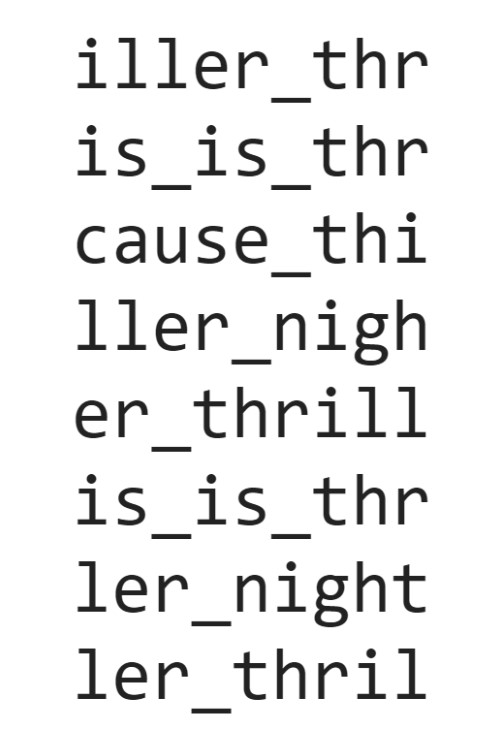
\includegraphics[scale=0.3]{images/fig1-1.jpg}
    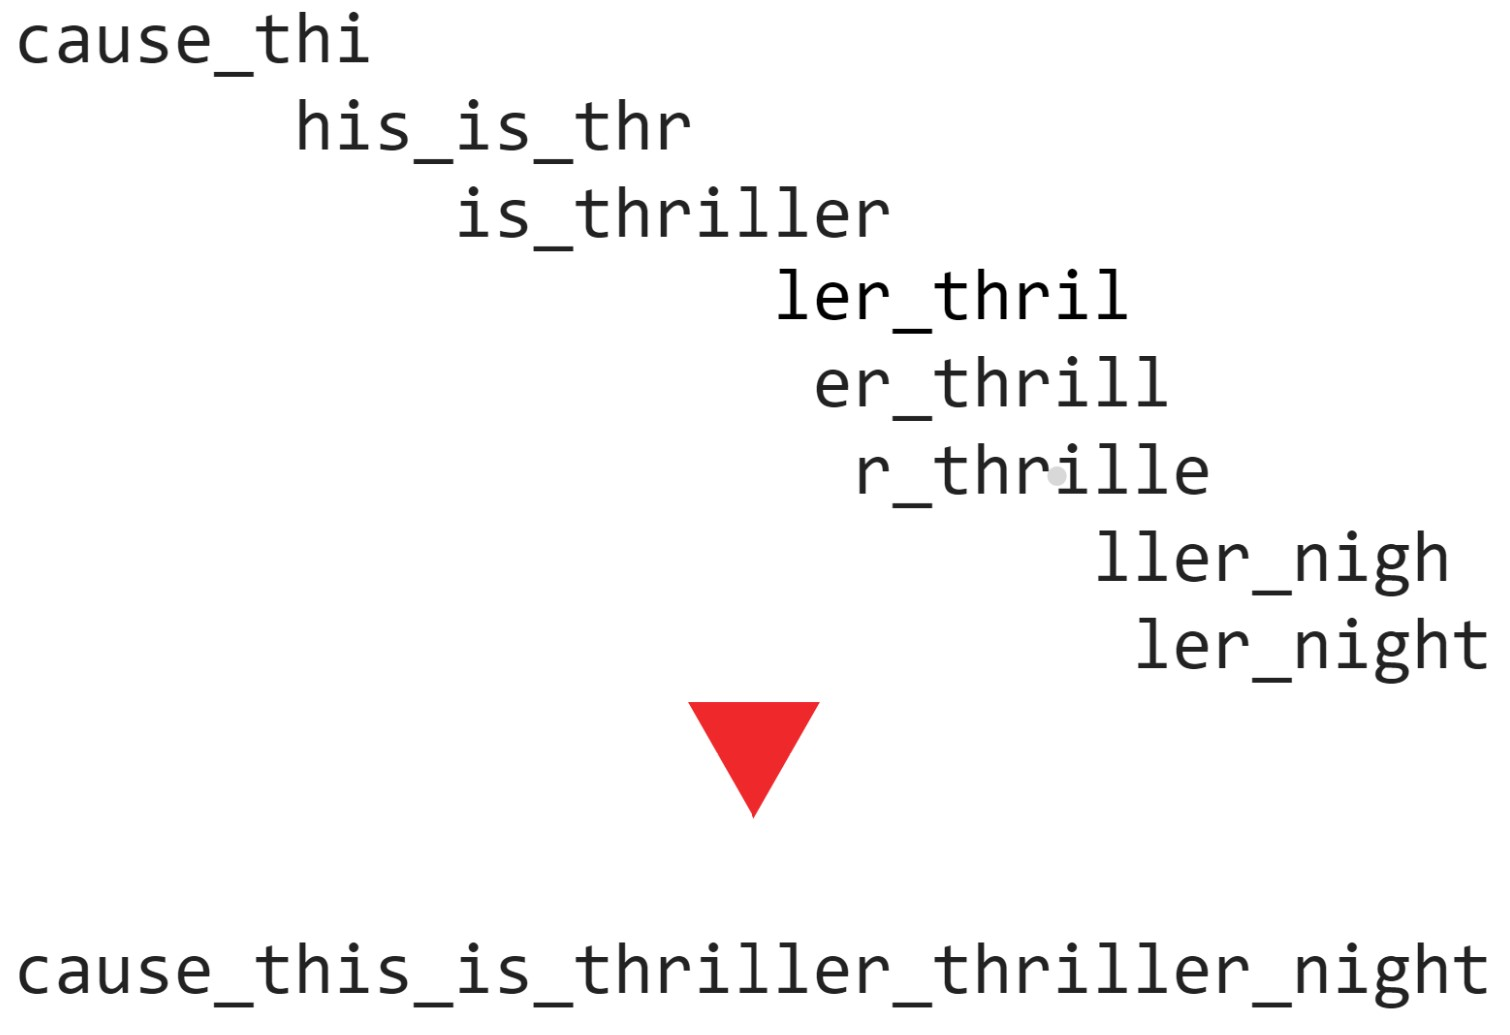
\includegraphics[scale=0.3]{images/fig1-2.jpg}
    \caption{An example of the read alignment problem being solved for a short sequence}
    \label{fig1}
  \end{figure}

  \subsection{The De Bruijn Graph}
  A De Bruijn graph is a directed graph that represents overlaps in sequences 
  of symbols.  The vertices of a De Bruijn graph consist of every permutation 
  of a fixed, finite alphabet.  Each edge corresponds do a difference of one 
  symbol between to sequences  A complete De Bruijn graph will have $a^b$ 
  vertices, where $a$ is the number of unique symbols in the alphabet and $b$ 
  is the sequence length\cite{wikipedia}. When using a De Bruijn graph to
  solve the assembly problem, not every permutation will appear.  It is also 
  possible that a given permutation will appear more than once. These graphs 
  are, therefore, partial De Bruijn multigraphs. De Bruijn graphs have an 
  extraordinary property when they have a unique Eulerian circuit. The
  eulerian circuit (the path that uses each edge exactly once) corresponds to
  the source sequence.  Finding the eulerian circuit of a De Bruijn graph 
  yields the source when loops are resolvable.

  \begin{algorithm}
    \caption{Inserting a read into graph}
    \begin{algorithmic}
      \IF {$prefix \in Nodes$}
        \STATE $leftNode \leftarrow Nodes[prefix]$
      \ELSE
        \STATE $leftNode \leftarrow Nodes[prefix] \leftarrow node(prefix)$
      \ENDIF
      \IF {$suffix \in Nodes$}
        \STATE $rightNode \leftarrow Nodes[suffix]$
      \ELSE
        \STATE $rightNode \leftarrow Nodes[suffix] \leftarrow node(suffix)$
      \ENDIF
    \end{algorithmic}
  \end{algorithm}

  \begin{algorithm}
    \caption{Compute Eulerian circuit}
    \begin{algorithmic}
      \STATE $circuit \leftarrow []$
      \IF {$eulerian$}
        \STATE $startNode \leftarrow next(Nodes)$
        \WHILE {$\bigm|startNode\bigm| > 0$}
          \STATE $add(circuit, startNode)$
          \STATE $startNode \leftarrow next(startNode)$
        \ENDWHILE
      \ENDIF
      \RETURN $circuit$
    \end{algorithmic}
  \end{algorithm}

  In algorithm one, prefix is defined as the sequence, in order, to be inserted
  minus the last element.  Suffix is defined in a similar manner: as the,
  sequence, in order, minus the first element.  Next is defined as the
  succeeding item in the order of nodes, or an arbitary node when no ordering exists.

  \begin{figure}[thpb]
    \centering
    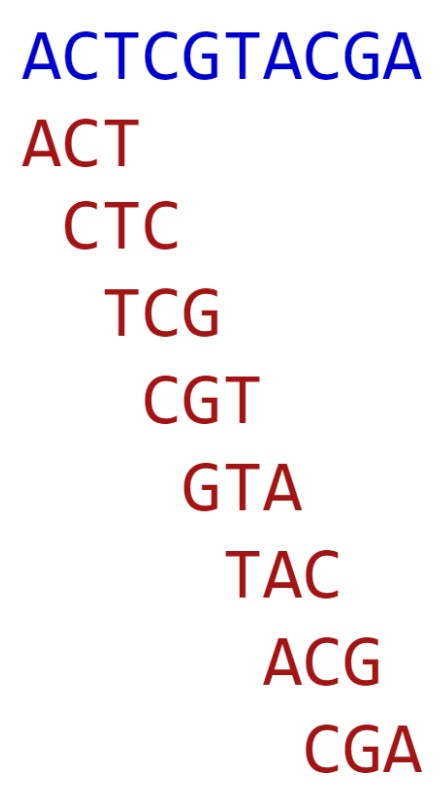
\includegraphics[scale=0.4]{images/fig2-1.jpg}
    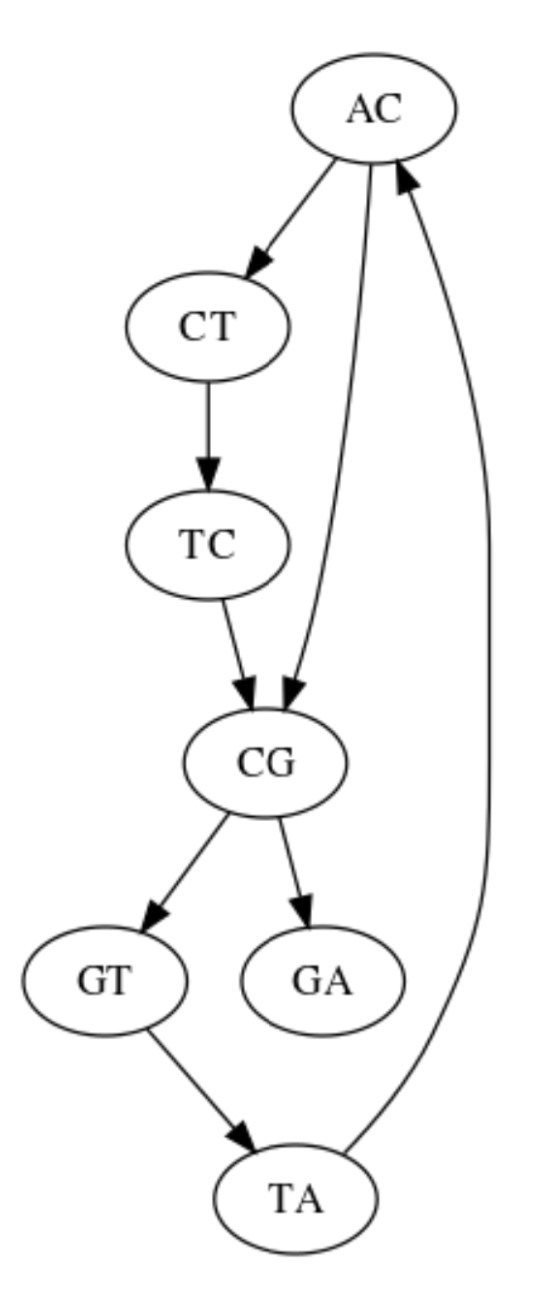
\includegraphics[scale=0.4]{images/fig2-2.jpg}
    \caption{An example graph of the reads of the sequence ACTCGTACGA}
    \label{fig2}
  \end{figure}

  Figure \ref{fig2} shows a short example of the De Bruijn graph of ACTCGTACGA.
  To simplify the example, each of the reads (shown in red) is of length three,
  though in practice these reads can be any length.  This graph can be read by
  simply starting at the head node (AC in this case) and adding it to the
  sequence.  Then the edges are followed (respecting their directionality) such
  that each edge is traveresed exactly once.  The last letter of each node
  (after the first) is added to the sequence.  In this example, the graph would
  be read as: AC-T-C-G-T-A-C-G-A.

  \break

  In figure \ref{fig3}, the sequence has three copies of the subsequence "AT".
  This creates an unresolvable loop in the graph.  This graph has two distict
  "loops" in its structure, yielding two valid eulerian circuits.  When read
  length is short, this kind of error is common \cite{langmead}.  This error can
  be resolved by increasing the length of the reads by one letter.  This yields
  figure \ref{fig4}, which has exactly one eulerian circuit.
  This issue is resolved becuase the "AT" subsequence that was causing problems
  now has more unique features associated with it which the graph can use to
  assemble unambiguiosly.


  \begin{figure}[thpb]
    \centering
    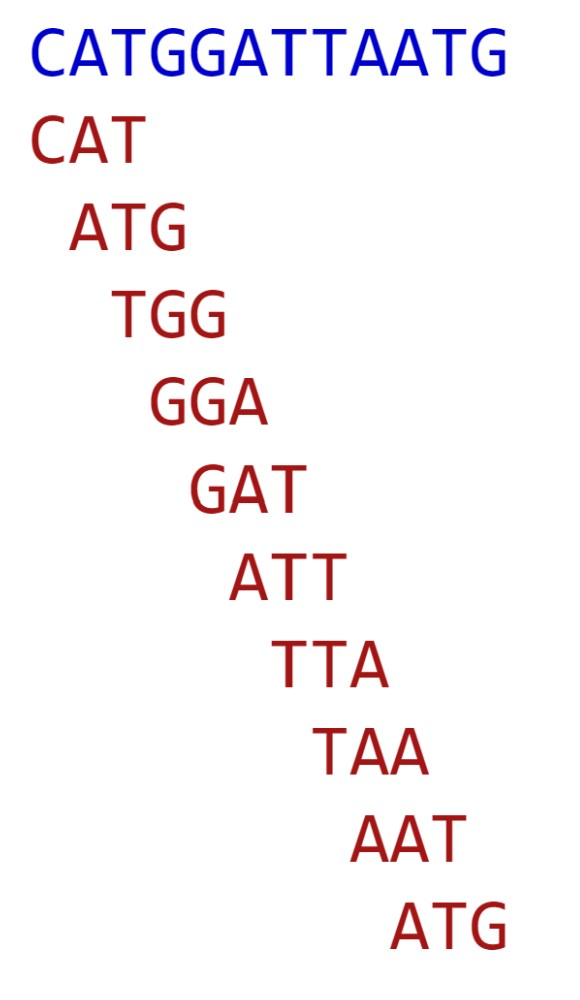
\includegraphics[scale=0.4]{images/fig3-1.jpg}
    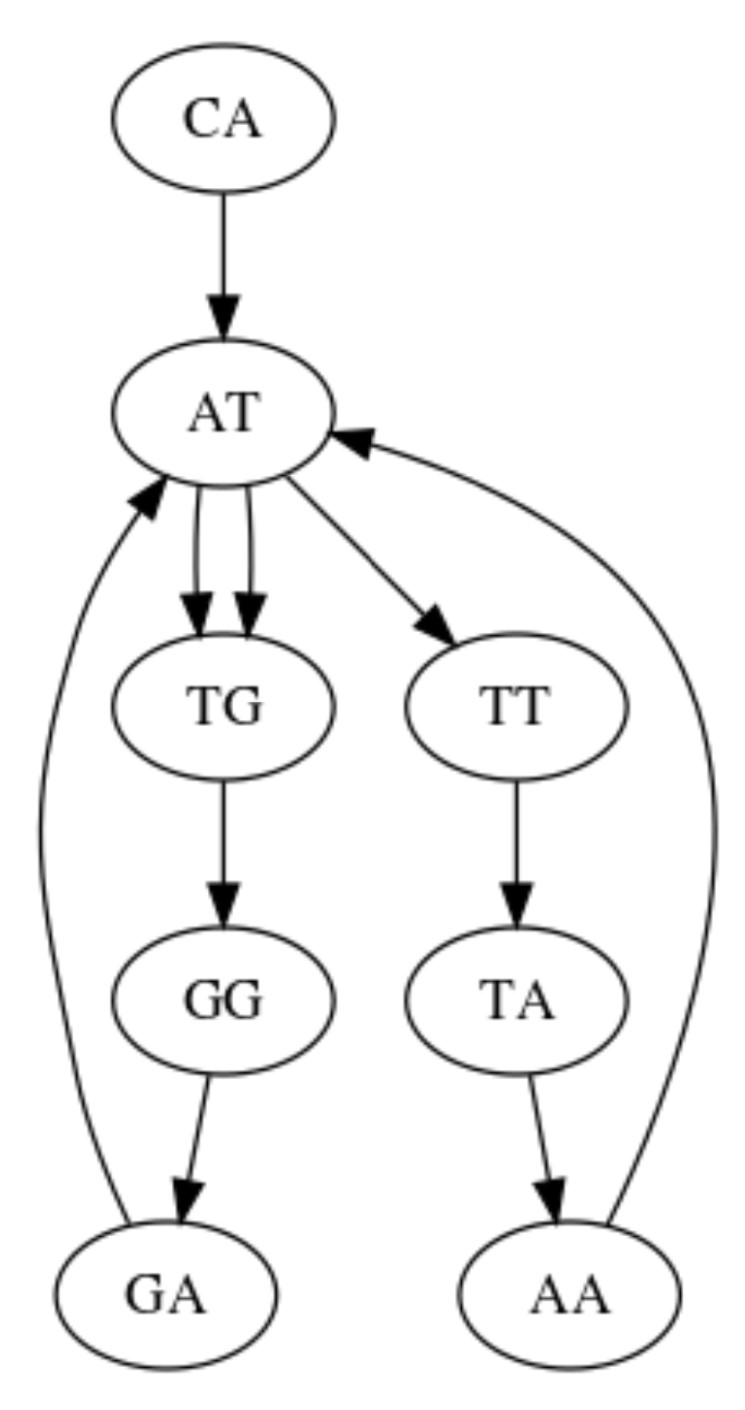
\includegraphics[scale=0.4]{images/fig3-2.jpg}
    \caption{An example of a graph with an unresolvable loop}
    \label{fig3}
  \end{figure}

  \begin{figure}[thpb]
    \centering
    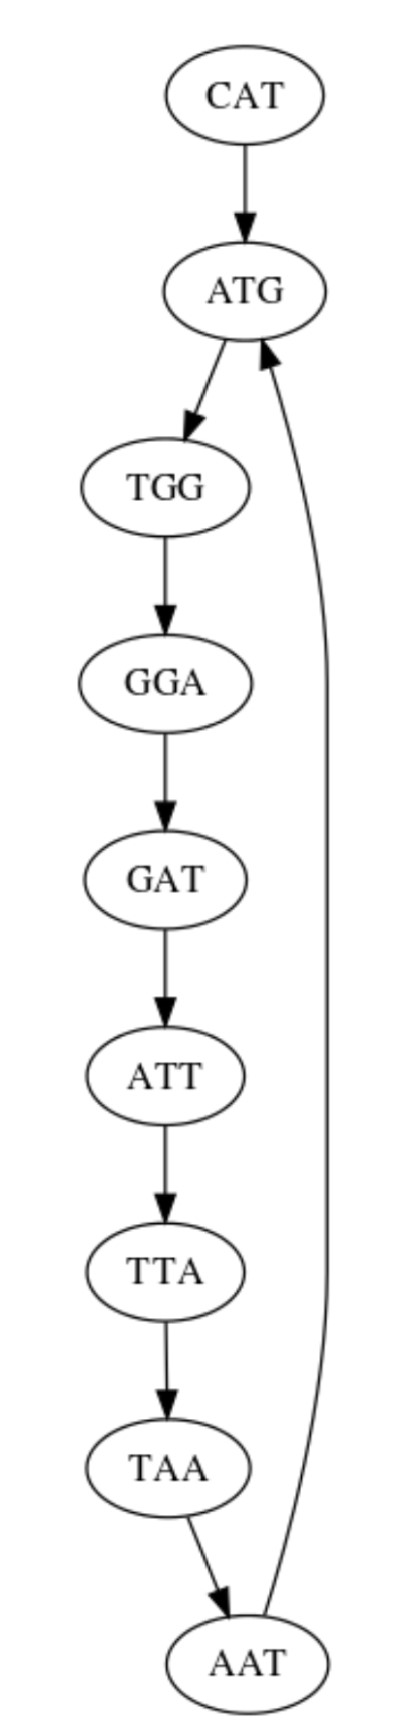
\includegraphics[scale=0.4]{images/fig4-1.jpg}
    \caption{A graph constructed of 4-mers}
    \label{fig4}
  \end{figure}

  \break

  Figure \ref{fig4} would be read as CATGGATTAATG, by stating at the first unbalanced
  node (CAT) and proceding to follow the loop as dictated by the eulerian circuit.
  
  \section{Read Length Optimization}
  \subsection{Data}
  As seen in figures \ref{fig3} and \ref{fig4}, read length has a direct effect
  on the resolvability of the De Bruijn graph.  In general, longer reads have
  more unique features useful for aligning \cite{langmead}.  Longer reads, however,
  require a larger De Bruijn graph.  Note that the number of vertices in a complete
  De Bruijn graph of length $b$ is $a^b$ where $a$ is the number of unique symbols
  in the alpahbet \cite{wikipedia}, in this case, four (A, C, T, and G).  For this
  reason, read lengths should be minimized.  The optimal read length for this task
  would be the minimum read length which still yields a single eulerian circuit.
  figures 5 and 6 plot average and maximum required read length
  over total genome length.  There is a clear logarithmic relationship between
  required read length and genome sequence length.  Figures 7 and 8
  again plot the average and maximum required read lengths versus total genome length,
  and again, the same logarithmic relationship is present.  It is clear that, when 
  the genome is small, very small reads will suffice.  This is expected because a 
  short sequence will have fewer repeated segments than a longer one.  This means
  that there will be fewer potential loops to resolve.  As the size of the genome
  increases, more unique patterns are nessasary to solve the allignment problem.

  \begin{figure}[thpb]
    \centering
    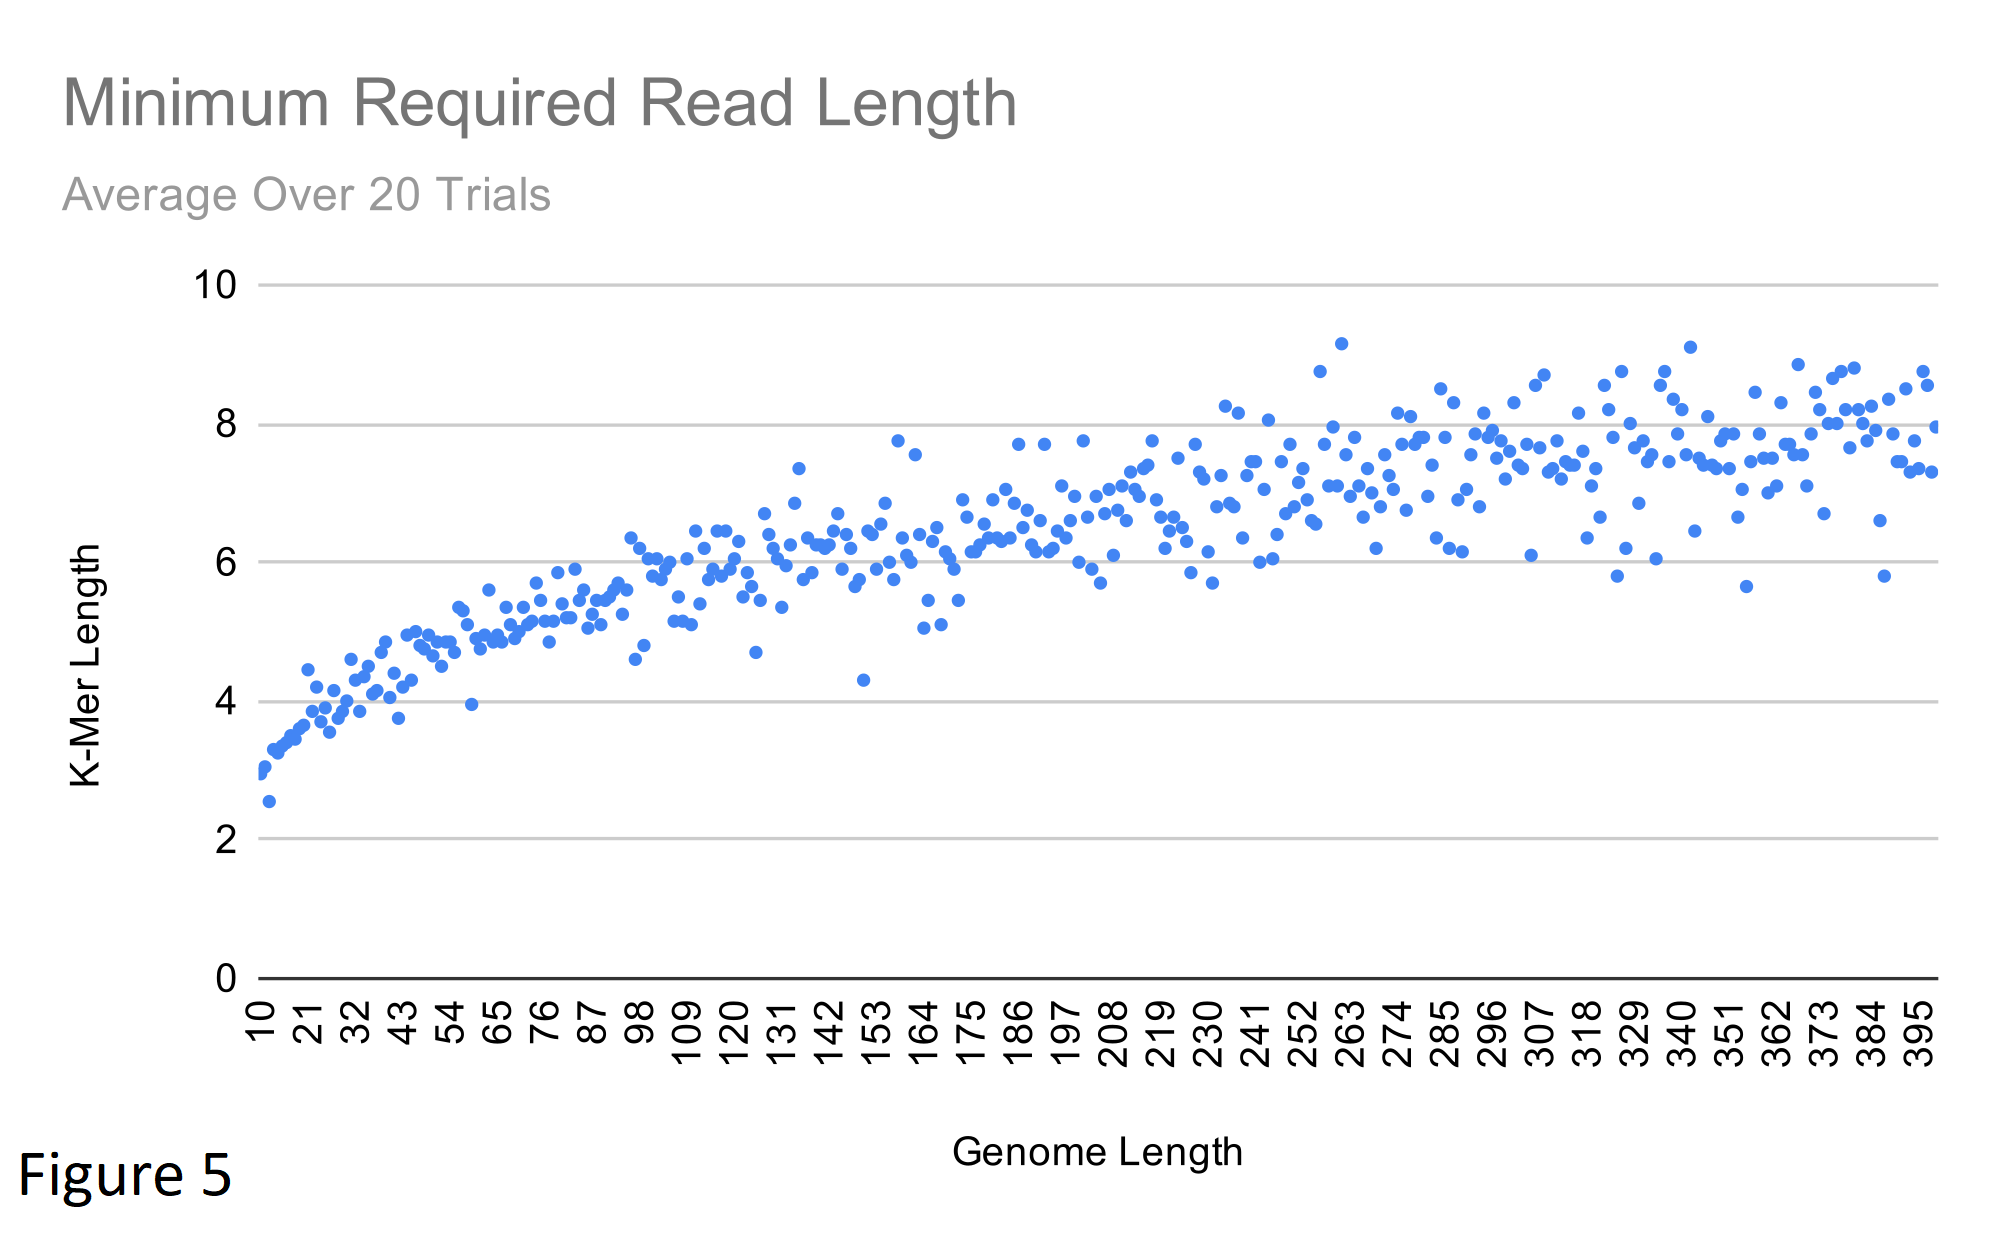
\includegraphics[scale=0.36]{images/Minimum_Required_Read_Length_(1).png}
    % \caption{Minimum Required Read Length (20 trial average)}
    \label{fig5}
  \end{figure}

  \begin{figure}[thpb]
    \centering
    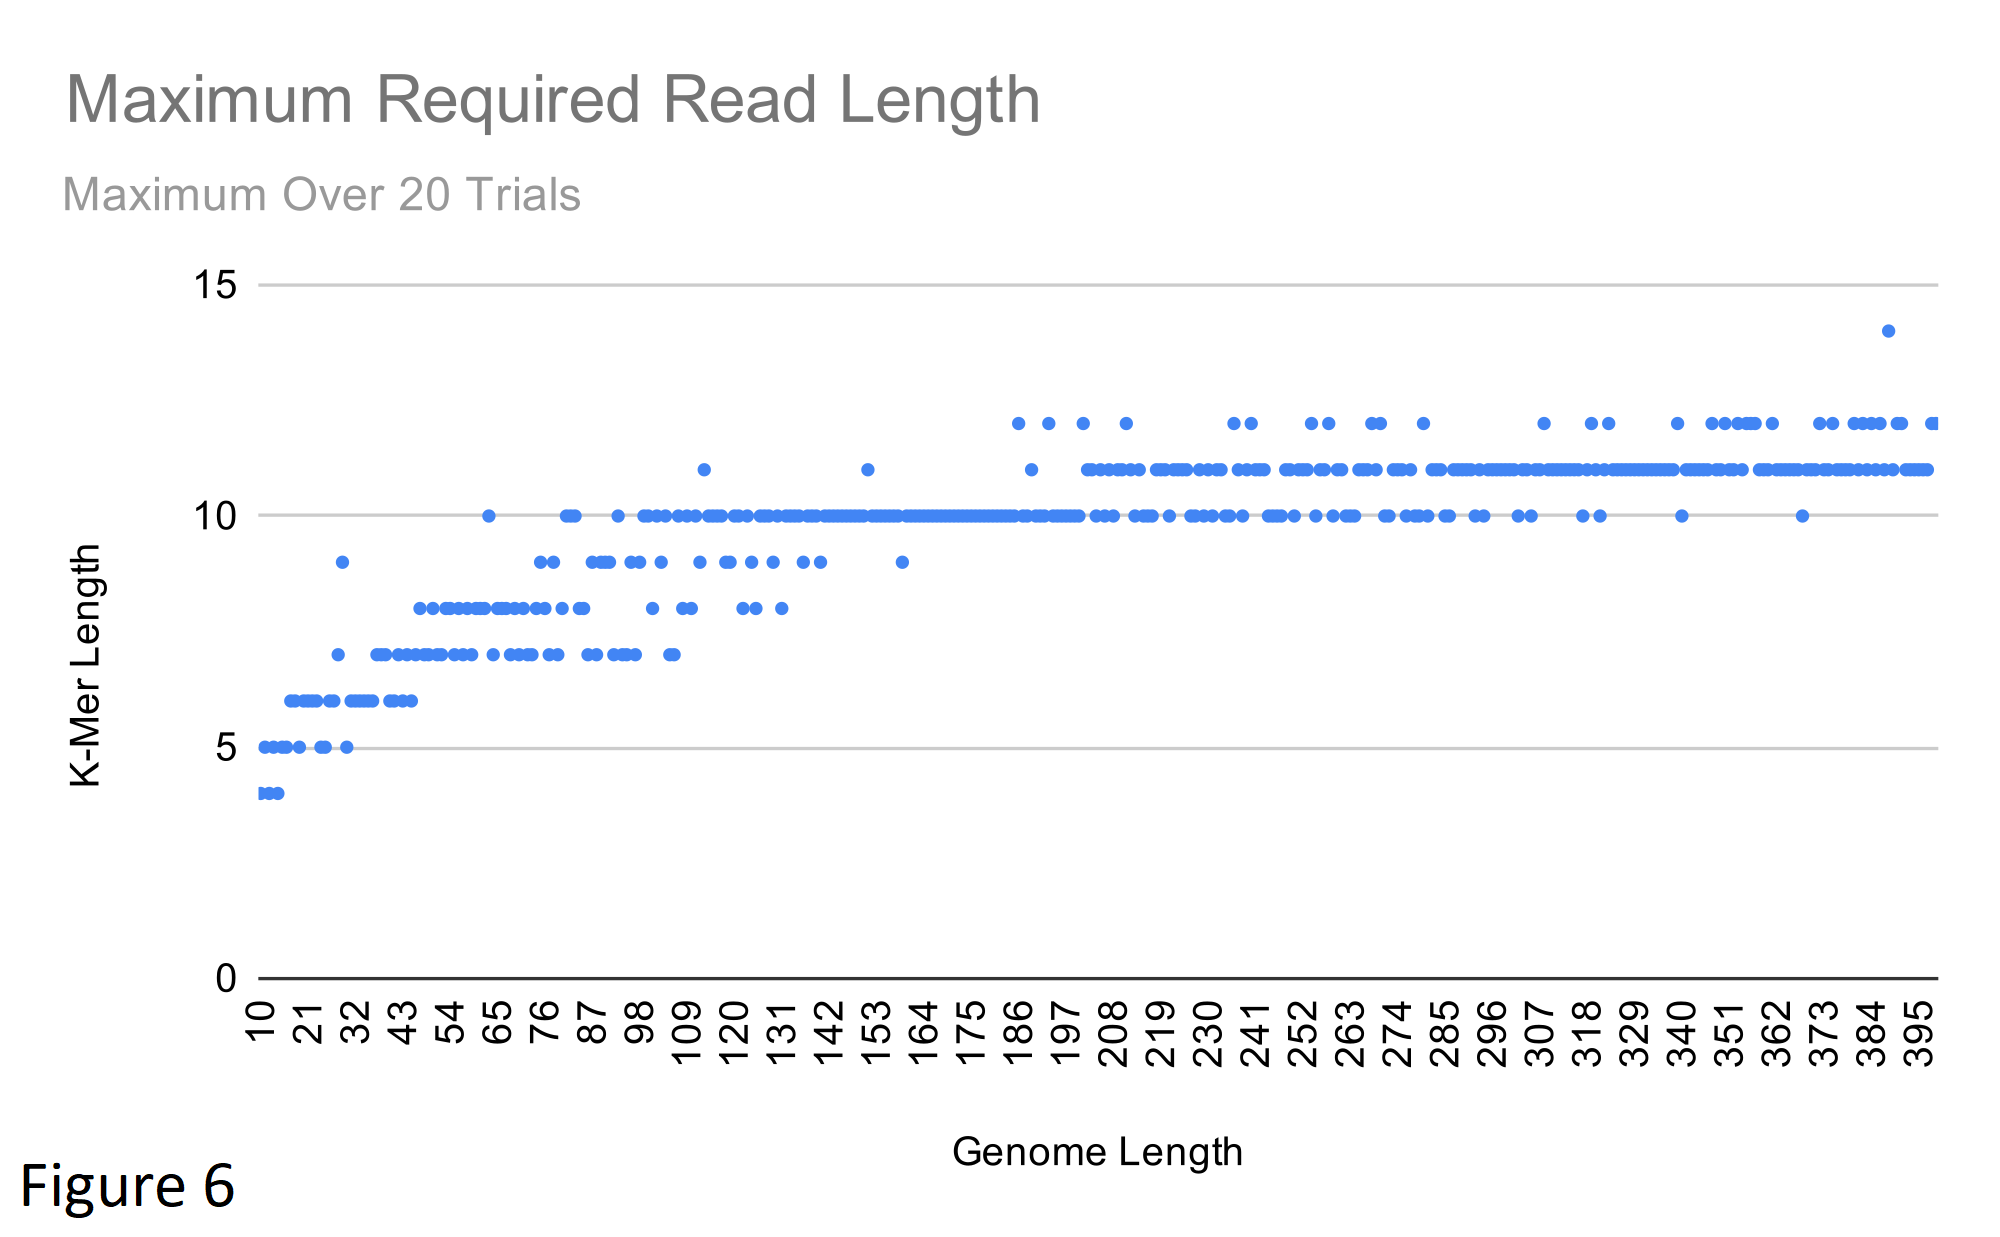
\includegraphics[scale=0.36]{images/Maximum_Required_Read_Length_(1).png}
    % \caption{Maximum Required Read Length (20 trial maximum)}
    \label{fig6}
  \end{figure}

  \begin{figure}[thpb]
    \centering
    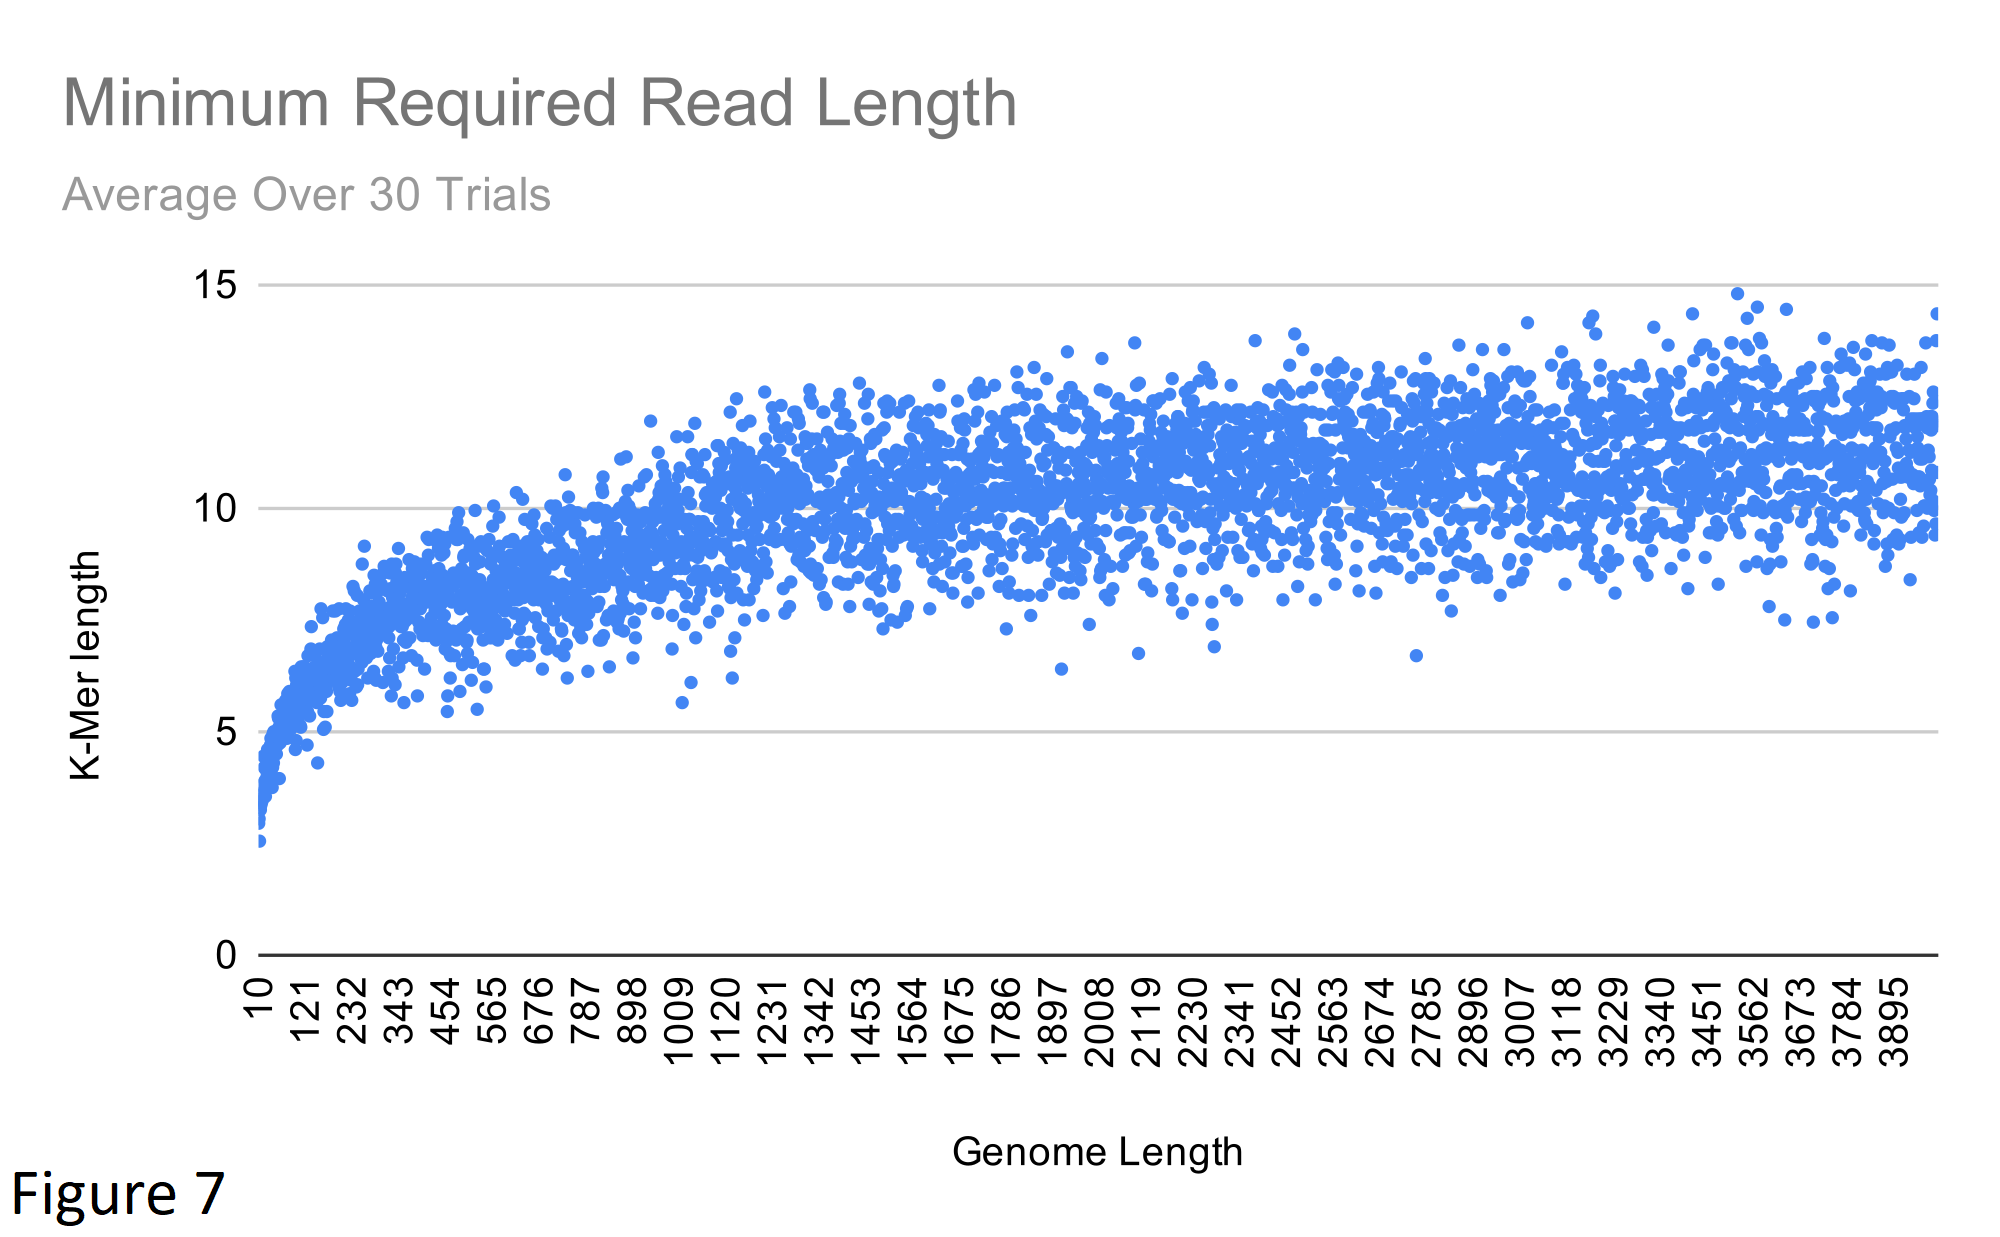
\includegraphics[scale=0.36]{images/Minimum_Required_Read_Length.png}
    % \caption{Minimum Required Read Length (30 trial average)}
    \label{fig7}
  \end{figure}

  \begin{figure}[thpb]
    \centering
    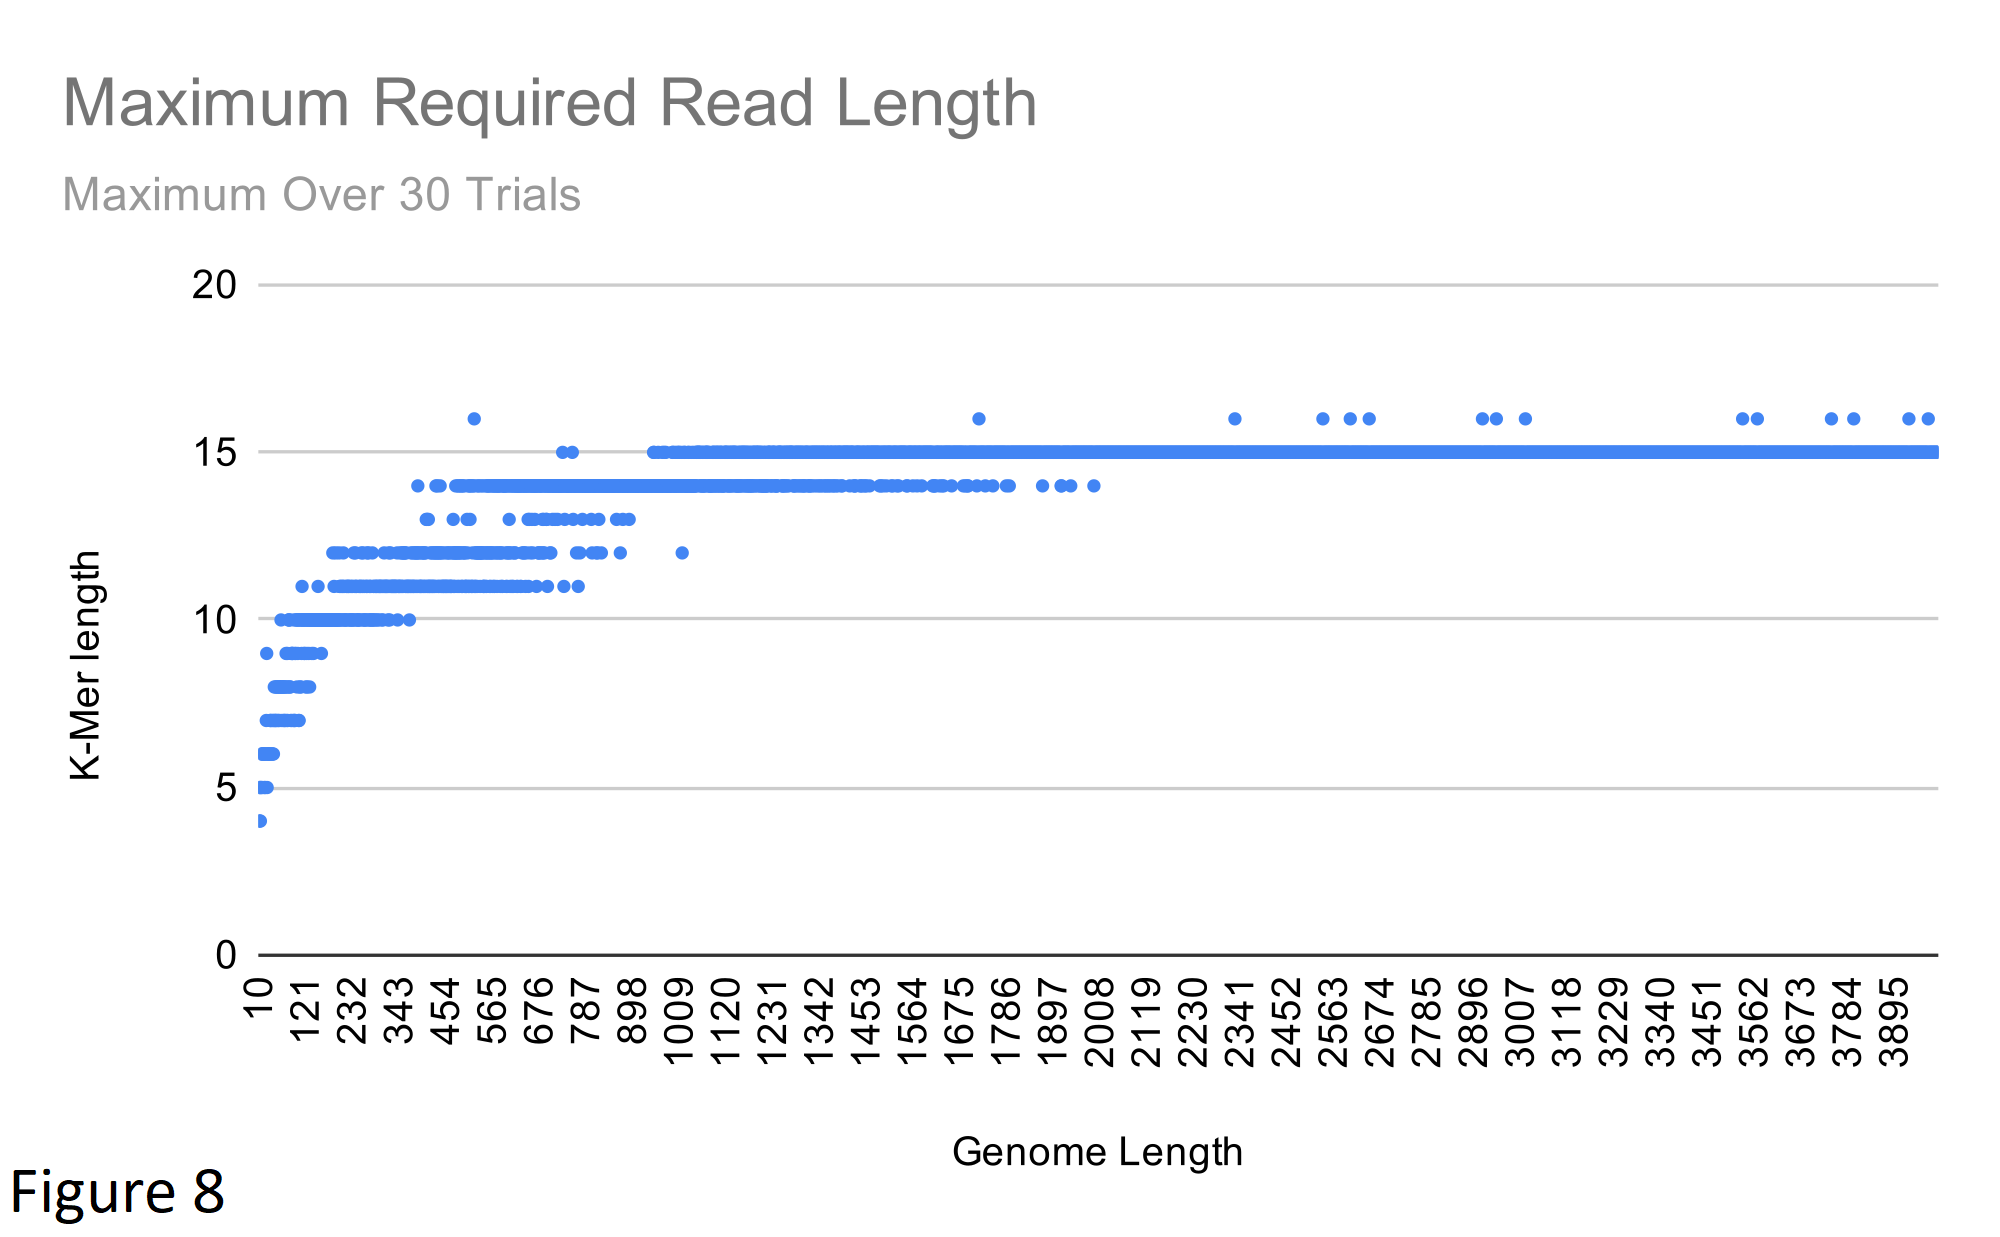
\includegraphics[scale=0.36]{images/Maximum_Required_Read_Length.png}
    % \caption{Maximum required Read Length (30 trial maximum)}
    \label{fig8}
  \end{figure}

  \subsection{Method}
  These data where collected by running the De Bruijn graph sequencer
  implementation on random segments of the HIV-1 virus \cite{ncbi.nlm.nih.gov}.
  To start a random segment of length $k$, where $k$ is "Genome Length" on the
  x-axis, is taken from the refrence genome.  The program then simulates
  "shotgun" reads, where random parts of the segment are read.  These reads are
  then shortened down to a length of two.  These shortened reads are fed into
  the De Bruijn graph assembler, which attempts to sequence the genome segment.
  If the sequencer is unable to produce a sequence, or it produces a sequence
  with an error, the result is thrown out and length of the shortened reads is
  increased by one.  This process reapeats until the sequencer can correctly
  sequence the genome segment.  This test is repeated twenty times for each
  genome length from ten to four-hundred.  These data are aggregated in figures
  5 and 6.  Figures 7 and 8 show the same
  process over thirty trials from k-mer length 10 to k-mer length 4000.

  \subsection{Conclusion}
  In this paper we have shown, that for genome lengths between 10 and 4000,
  there exists a logarithmic relationship between the length of the genome and the
  minimum avgerage read length.  Applying a logarithmic regression to these data yields
  $1.51\ln{x}$ with $R^2 = 0.641$.  We can say that, for genome sizes between 10 and 4000,
  the function $\mathcal{K}$ which takes a genome length and returns the optimal read
  length is $\mathcal{K}(x) \approx 1.51 \ln{x}$.  In the future, metrics like the one
  proposed in this paper could be used to greatly reduce both memory and time costs of
  sequencing an entire genome.  Combined with tequinques like De Bruijin graph gene compression
  \cite{dazdomnguez2019simulating}, better scaling assemblers \cite{10.1093/bioinformatics/bty648}
  and other techniques like edge minimization \cite{baier2019edge} personalized medicine 
  and personal gene ownership could become a reality.

  \newpage

  \bibliographystyle{unsrt}
  \bibliography{refrence}

\end{document}